\documentclass[crop,tikz]{standalone}

\usepackage{tikz}
\usepackage{anyfontsize}

\usetikzlibrary{bending}
\usetikzlibrary{arrows.meta}
\begin{document}
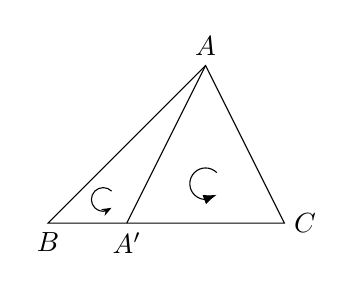
\begin{tikzpicture}

\draw (0,0) -- (3,0) -- (2,2) -- cycle;
\draw (1,0) -- (2,2);
\node [below] at (0,0) {$B$};
\node [above] at (2,2) {$A$};
\node [below] at (1,0) {$A'$};
\node [right] at (3,0) {$C$};

\draw [-Latex] ([shift=(45:0.2)]2,0.5) arc [radius=0.2, start angle=45, end angle= 315];
\draw [arrows = {-Stealth[scale=0.75]}] ([shift=(45:0.15)]0.7,0.3) arc [radius=0.15, start angle=45, end angle= 315];

\end{tikzpicture}
\end{document}